% Author: Rasmus Pank Roulund
\documentclass{minimal}
\usepackage{tikz}
\usetikzlibrary{arrows,calc}
\usepackage{relsize}
\newcommand\LM{\ensuremath{\mathit{LM}}}
\newcommand\IS{\ensuremath{\mathit{IS}}}
\begin{document}

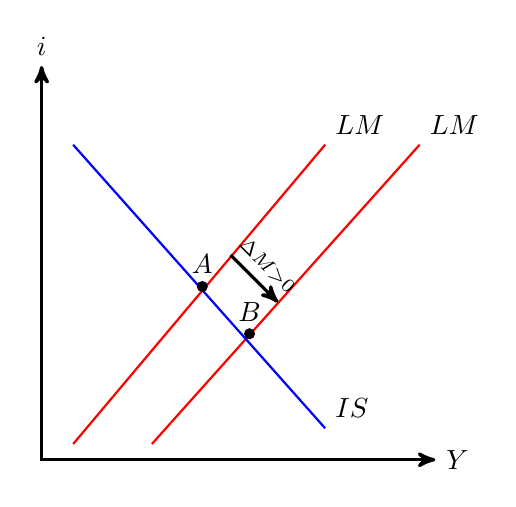
\begin{tikzpicture}[
        scale=2,
        IS/.style={blue, thick},
        LM/.style={red, thick},
        axis/.style={very thick, ->, >=stealth', line join=miter},
        important line/.style={thick}, dashed line/.style={dashed, thin},
        every node/.style={color=black},
        dot/.style={circle,fill=black,minimum size=4pt,inner sep=0pt,
            outer sep=-1pt},
    ]
    % axis
    \draw[axis,<->] (2.5,0) node(xline)[right] {$Y$} -|
                    (0,2.5) node(yline)[above] {$i$};
	
	%LM
	\draw[important line, red, xshift=.1cm]
	            (.1,.1) coordinate (es) -- (1.7,2) coordinate (ee)
	            node [above right] {$LM$};
	
	%LM after shift
	\draw[important line, red, xshift=.1cm]		         
	   (.6,.1) coordinate (es) -- (2.3,2) coordinate (ee)
	   node [above right] {$LM$};
	
	%IS
	\draw[important line, blue, xshift=.1cm]
	            (.1,2) coordinate (es) -- (1.7,.2) coordinate (ee)
	            node [above right] {$IS$};
	
	\node[dot,label=above:$A$] at (1.02,1.1) (int1) {};
	\node[dot,label=above:$B$] at (1.32,.8) (int1) {};
	
	\draw[->, very thick, black, >=stealth']
       (1.2,1.3) -- (1.5,1)
        node[sloped, above, midway] {$\mathsmaller{\Delta M > 0}$};
    % IS-LM diagram
    %\draw[LM] (0.8,0.3) coordinate  (LM_1)  (1.8,1.8)
     %   coordinate (LM_2) node[above] {\LM};
    %\draw[IS] (0.2,1.8) coordinate (IS_1) parabola[bend at end]
     %    (1.8,.3) coordinate (IS_2) node[right] {\IS};
    %Intersection is calculated "manually" since Tikz does not offer
    %intersection calculation for parabolas
    
    %shifted IS-LM diagram
    %\draw[xshift=.7cm, LM, red!52] (0.2,0.2) parabola (1.8,1.7)
     %   node[above] {\LM'};
    %\draw[xshift=.4cm, yshift=.3cm, IS, blue!60] (0.2,1.8)
     %   parabola[bend at end] (1.8,.3)
    %    node[right] {\IS'};
    %Intersection of shifted IS-LM
    %\path[xshift=.36cm, yshift=.35cm] (.98,.7)
     %   node[dot,label=above:{$B$}] (int2) {};
    %\path[xshift=.805cm] (1,.68) node[dot,label=above:$C$] (int3) {};
    %arrows between intersections
    %\draw[->, very thick, black, >=stealth']
      %  ($(int1)+1/2*(-.80,1)$) -- ($(int2)+1/2*(-.8,1)$)
     %   node[sloped, above, midway] {$\mathsmaller{\Delta G > 0}$};
    %\draw[->, very thick, black, >=stealth']
     %   ($(int2)+2*(.14,.2)$) -- ($(int2)!.2cm!270:(int2)+(.9,0)$)
    %    node[sloped,above, midway] {$\mathsmaller{\Delta M>0}$};
        
    

\end{tikzpicture}
\end{document}